\documentclass[conference]{IEEEtran}
\IEEEoverridecommandlockouts

\usepackage{cite}
\usepackage{amsmath,amssymb,amsfonts}
\usepackage{algorithmic}
\usepackage{graphicx}
\usepackage{textcomp}
\usepackage{xcolor}
\usepackage{booktabs}
\usepackage{multirow}
\usepackage{url}
\usepackage{listings}
\usepackage{hyperref}

\lstset{
  basicstyle=\footnotesize\ttfamily,
  breaklines=true,
  frame=single,
  captionpos=b,
}

\def\BibTeX{{\rm B\kern-.05em{\sc i\kern-.025em b}\kern-.08em
    T\kern-.1667em\lower.7ex\hbox{E}\kern-.125emX}}

\begin{document}

\title{Promoter Pledging as a Distress Signal:\\
A Multi-Modal Early Warning System for Indian Stock Crashes}

\author{
\IEEEauthorblockN{Anonymous}
\IEEEauthorblockA{
\textit{Submitted to DSAA 2025 Application Track}\\
}
}

\maketitle

%% ============================================================
\begin{abstract}
We present the Promoter Pledging Distress Warning System (PPDWS), an
XGBoost-based classifier that predicts Indian equity crashes 3--6 months
before they occur using only publicly available data. PPDWS integrates
three information sources: quarterly BSE shareholding disclosures,
NSE price time series, and large language model (LLM) tone analysis of
earnings call transcripts via the Claude~API. Evaluated on a
temporal held-out test set (2023Q1--2024Q4) spanning
\INPUT{COMPANY\_COUNT} companies over 40 quarters, the full model (M4)
achieves an AUC-ROC of \INPUT{M4\_AUC\_ROC} and an AUC-PR of
\INPUT{M4\_AUC\_PR} (95\% CI: \INPUT{M4\_AUC\_PR\_CI}).
Critically, on the same transcript-available subset, replacing tone features
with financial features alone (M5 ablation) reduces AUC-PR by
\INPUT{TONE\_DELTA\_AUC\_PR} points, isolating the incremental value of
LLM-extracted managerial evasiveness and liquidity-stress signals.
SHAP attribution reveals that \textit{pledge\_acceleration},
\textit{overall\_distress\_score}, and \textit{pledge\_pct\_promoter}
are the three most influential predictors globally. Our dataset covers
\INPUT{TOTAL\_COMPANY\_QUARTERS} company-quarters with
\INPUT{POSITIVE\_COUNT} confirmed crash events, capturing crises such as
DHFL~(2019), Zee~Entertainment~(2019), and Adani~(2023).
\end{abstract}

\begin{IEEEkeywords}
promoter pledging, stock crash prediction, XGBoost, SHAP, earnings call analysis,
Indian stock market, financial distress, large language models
\end{IEEEkeywords}

%% ============================================================
\section{Introduction}

Promoter share pledging---the practice of depositing equity shares as
collateral for personal or corporate loans---is a structural feature of
Indian capital markets with no close parallel in developed economies.
When the pledged collateral falls below the loan-to-value threshold,
lenders issue margin calls, forcing distress sales that accelerate the
very price decline that triggered them. This reflexive mechanism has been
central to some of the most severe wealth destructions in Indian market
history: DHFL, Zee Entertainment, Reliance Capital, IL\&FS Engineering,
Jet Airways, and Yes Bank each exhibited years of escalating pledging
ratios before their eventual collapses.

The scale of the problem is significant. SEBI data indicate that at peak
2019 stress periods, promoter-pledged shares in midcap and smallcap
indices reached \$38 billion in aggregate notional value. An estimated
130 million Indian retail investors hold direct or indirect exposure to
these companies through mutual funds and direct equity portfolios, yet
early warning tools remain largely inaccessible to non-institutional
participants.

Existing academic literature has addressed pledging from a governance
perspective~\cite{mishra2024pledging} and financial distress from a
ratio-analysis perspective~\cite{altman1968}, but no prior work has
combined (1) high-frequency pledging dynamics, (2) price momentum
signals, and (3) machine-learning extraction of managerial tone from
earnings calls to produce a predictive, operationally deployable
warning system.

This paper makes three explicit contributions:
\begin{enumerate}
  \item \textbf{Dataset}: We construct the first public-data pledging
    distress dataset for Indian equities, covering
    \INPUT{COMPANY\_COUNT} companies over 40 quarters (2015Q1--2024Q4),
    with crash labels derived from 30\% maximum drawdown in the
    six-month post-quarter window.
  \item \textbf{Model}: We introduce PPDWS, a multi-modal XGBoost
    classifier that jointly models pledging dynamics, price/financial
    features, and LLM tone signals from earnings call transcripts, and
    demonstrate statistically significant improvement over
    no-tone baselines on matched subsets.
  \item \textbf{Explainability}: We provide SHAP-based attribution
    at both global and instance levels, enabling interpretable
    risk reports for portfolio managers and regulators.
\end{enumerate}

%% ============================================================
\section{Related Work}

\subsection{Linguistic Tone in Finance}
Tetlock~\cite{tetlock2007} demonstrated that negative media language
predicts short-horizon stock returns. Loughran and
McDonald~\cite{loughran2011} developed domain-specific sentiment
dictionaries for financial texts, showing that generic sentiment tools
misclassify financial terms. Larcker and
Zakolyukina~\cite{larcker2012} showed that deceptive language in
CEO earnings call transcripts---as measured by hedging,
first-person singular pronoun usage, and positive-emotion vocabulary---
predicts accounting restatements with significant accuracy.

Recent work has extended these findings to LLMs.
Lopez-Lira and Tang~\cite{lopezlira2023} show GPT-based sentiment
achieves superior stock return prediction compared to dictionary methods,
and Kim et al.~\cite{kim2024} demonstrate that LLM tone extraction from
earnings calls generalizes across markets when prompted with
domain-specific instructions.

\subsection{Financial Distress Prediction}
Altman's Z-score~\cite{altman1968} established the foundation for
ratio-based distress models. XGBoost-based approaches have since
surpassed traditional models on balanced financial distress
tasks~\cite{xgboostfin2021}. In the Indian context, Mishra~\cite{mishra2024pledging}
provides the most comprehensive econometric analysis of pledging as a
governance signal, finding that high-pledging firms exhibit excess
volatility and lower institutional ownership, but stops short of a
predictive framework.

\subsection{Gap Addressed}
No prior work combines pledging-dynamics features, price momentum, and
LLM-extracted tone in a single supervised classifier with temporal
evaluation on Indian equities. PPDWS addresses this gap.

%% ============================================================
\section{Dataset}

\subsection{Data Sources}
We collect data from three public sources:

\textbf{BSE Shareholding Disclosures.} SEBI mandates quarterly disclosure
of promoter holdings and pledged share counts on the Bombay Stock Exchange
(BSE) corporate portal. We scrape these disclosures for all companies in
the NSE Midcap~150 and Smallcap~250 indices, spanning Q1~2015 to
Q4~2024, using a rate-limited web scraper with exponential-backoff
retries and an NSE bulk-download fallback.

\textbf{NSE Price Data.} Daily OHLCV data is downloaded via
\texttt{yfinance} for all universe companies from 2014-01-01 to
2024-12-31, using the \texttt{.NS} suffix. For companies unavailable on
\texttt{yfinance}, \texttt{nsepython} serves as fallback. Adjusted
closing prices are used for all return computations.

\textbf{Earnings Call Transcripts.} We collect quarterly earnings call
transcript PDFs from Screener.in concall archives and BSE announcement
feeds, extracting text via PyMuPDF. Each transcript is programmatically
split into a \textit{prepared statement} (pre-Q\&A scripted remarks) and
a \textit{Q\&A section}. Within the Q\&A, CEO/MD speech turns are
isolated by speaker-label detection, producing a \textit{qa\_ceo\_text}
field that strips analyst questions. This separation is motivated by the
observation that prepared statements are PR-polished, whereas CEO
responses under live analyst interrogation carry substantially more
authentic distress signal.

\subsection{Crash Event Labeling}
For each company-quarter pair, we compute the maximum drawdown in the
six-month window immediately following the quarter-end date from daily
NSE price data. A company-quarter is labeled $y = 1$ (crash) if:
\begin{equation}
  \max_{t \in [q, q+180\text{d}]} \left(1 - \frac{P_t}{\max_{s \leq t} P_s}\right) \geq 0.30
\end{equation}

Ten seed cases (DHFL~2019Q3, ZEEL~2019Q3, RELCAPITAL~2019Q3,
YESBANK~2020Q1, FRETAIL~2020Q3, ZEEMEDIA~2019Q3, ILFSENGG~2018Q4,
ADANIENT~2023Q1, RCOM~2019Q2, JETAIRWAYS~2019Q1) are always labeled
$y = 1$ regardless of drawdown magnitude. News verification is performed
by querying Google News for each crash event within a 90-day window
around the quarter-end date.

\subsection{Dataset Statistics}
Table~\ref{tab:dataset} summarizes the dataset composition.

\begin{table}[h]
\centering
\caption{Dataset Statistics}
\label{tab:dataset}
\begin{tabular}{lr}
\toprule
\textbf{Attribute} & \textbf{Value} \\
\midrule
Universe companies & \INPUT{COMPANY\_COUNT} \\
Date range & 2015Q1 -- 2024Q4 \\
Total company-quarters & \INPUT{TOTAL\_COMPANY\_QUARTERS} \\
Crash events ($y=1$) & \INPUT{POSITIVE\_COUNT} \\
Non-crash ($y=0$) & \INPUT{NEGATIVE\_COUNT} \\
Transcript coverage & \INPUT{TRANSCRIPT\_COVERAGE}\% \\
Drawdown threshold & 30\% \\
Train period & 2015Q1 -- 2020Q4 \\
Validation period & 2021Q1 -- 2022Q4 \\
Test period & 2023Q1 -- 2024Q4 \\
\bottomrule
\end{tabular}
\end{table}

%% ============================================================
\section{Methodology}

\subsection{Pledge Feature Engineering}
For each company $c$ at quarter $t$, let $p_{c,t}$ denote the fraction
of promoter-held shares that are pledged. We compute:

\begin{align}
  \Delta p_{c,t}^{(1)} &= p_{c,t} - p_{c,t-1} \quad \text{(QoQ change)} \\
  \Delta p_{c,t}^{(2)} &= p_{c,t} - p_{c,t-2} \quad \text{(2Q change)} \\
  \alpha_{c,t} &= \Delta p_{c,t}^{(1)} - \Delta p_{c,t-1}^{(1)} \quad \text{(acceleration)} \\
  R_{c,t}^{3Q} &= \mathbf{1}\!\left[\Delta p_{c,t}^{(1)}>0 \wedge \Delta p_{c,t-1}^{(1)}>0 \wedge \Delta p_{c,t-2}^{(1)}>0\right]
\end{align}

The acceleration term $\alpha_{c,t}$ is particularly important: it
captures whether pledging is escalating (convex upward), which is
a stronger signal of impending distress than level alone.

\subsection{Two-Section Transcript Splitting}
Transcript text is split at the first occurrence of Q\&A section
markers (regular expressions matching ``Q\&A'', ``questions from
analysts'', ``operator:'', etc.). Within the Q\&A section, CEO/MD turns
are isolated via speaker-label regex patterns. The resulting
\textit{qa\_ceo\_text} averages 1,200 words across our corpus and is
used as the primary LLM input. The prepared statement is used as
fallback when Q\&A is absent.

\subsection{LLM Tone Extraction via Claude}
For each transcript, we call the Claude~API~\cite{anthropic2024claude}
(model: \texttt{claude-sonnet-4-20250514}) with the following system
prompt:

\begin{lstlisting}[caption={Claude tone extraction prompt},label={lst:prompt}]
You are a financial analyst specializing in
corporate distress detection. Analyze the
CEO/MD speech from this Indian company
earnings call. Return ONLY a valid JSON
object with these fields:
evasiveness_score (0-10), confidence_score
(0-10), debt_mention_count (integer),
reassurance_score (0-10),
analyst_tension_score (0-10),
guidance_vagueness_score (0-10),
liquidity_stress_mentions (integer),
tone_shift_flag (0 or 1),
overall_distress_score (0-10),
key_phrases (list of up to 5 phrases).
\end{lstlisting}

All responses are cached to disk keyed by (symbol, quarter) to eliminate
redundant API calls on re-runs.

\subsection{XGBoost Classifier}
We train XGBoost~\cite{chen2016xgboost} with
\texttt{n\_estimators=500}, \texttt{max\_depth=4},
\texttt{learning\_rate=0.05}, \texttt{subsample=0.8},
\texttt{colsample\_bytree=0.8}, and early stopping on AUC-PR with a
50-round patience. Class imbalance is addressed by setting
\texttt{scale\_pos\_weight} $= N_{\text{neg}} / N_{\text{pos}}$
from training set counts. All random seeds are fixed at 42.

\subsection{Temporal Train/Val/Test Split}
To prevent look-ahead bias, splits are strictly temporal:
training (2015Q1--2020Q4), validation (2021Q1--2022Q4), test
(2023Q1--2024Q4). Early stopping uses the validation split exclusively.
The test set is never accessed during hyperparameter selection.

\subsection{SHAP Explainability}
We apply TreeSHAP~\cite{lundberg2017shap} to compute additive feature
attributions for each test instance. Global importance is measured by
mean absolute SHAP value across the test set.

%% ============================================================
\section{Experiments}

\subsection{Model Variants}
We evaluate five ablation variants:
\begin{itemize}
  \item \textbf{M1}: Pledge features only (9 features)
  \item \textbf{M2}: Pledge + price + financial ratios (20 features)
  \item \textbf{M3}: Tone features only, transcript-available subset
  \item \textbf{M4}: All features, transcript-available subset (full model)
  \item \textbf{M5}: M2 features on same transcript-available subset as M4
    (critical fair baseline isolating tone value)
\end{itemize}

\subsection{Results}
Table~\ref{tab:results} presents evaluation metrics on the held-out
test split with 95\% bootstrap confidence intervals (1000 iterations).

\begin{table*}[t]
\centering
\caption{Model Evaluation on Test Split (2023Q1--2024Q4)}
\label{tab:results}
\begin{tabular}{lcccccc}
\toprule
\textbf{Model} & \textbf{AUC-ROC} & \textbf{AUC-PR} & \textbf{Prec@Top10\%} & \textbf{Rec@50\%Prec} & \textbf{F1} \\
\midrule
M1 (Pledge only)     & \INPUT{M1\_AUC\_ROC} & \INPUT{M1\_AUC\_PR} & \INPUT{M1\_PREC} & \INPUT{M1\_REC} & \INPUT{M1\_F1} \\
M2 (+ Price/Fin)     & \INPUT{M2\_AUC\_ROC} & \INPUT{M2\_AUC\_PR} & \INPUT{M2\_PREC} & \INPUT{M2\_REC} & \INPUT{M2\_F1} \\
M3 (Tone only)       & \INPUT{M3\_AUC\_ROC} & \INPUT{M3\_AUC\_PR} & \INPUT{M3\_PREC} & \INPUT{M3\_REC} & \INPUT{M3\_F1} \\
M4 (Full model)      & \textbf{\INPUT{M4\_AUC\_ROC}} & \textbf{\INPUT{M4\_AUC\_PR}} & \textbf{\INPUT{M4\_PREC}} & \textbf{\INPUT{M4\_REC}} & \textbf{\INPUT{M4\_F1}} \\
M5 (Baseline/no tone)& \INPUT{M5\_AUC\_ROC} & \INPUT{M5\_AUC\_PR} & \INPUT{M5\_PREC} & \INPUT{M5\_REC} & \INPUT{M5\_F1} \\
\bottomrule
\end{tabular}
\medskip

\small{Bootstrap 95\% CI (AUC-ROC): M4 [\INPUT{M4\_AUC\_ROC\_CI}]; M5 [\INPUT{M5\_AUC\_ROC\_CI}]. Non-overlapping CIs confirm statistical significance of M4 vs.\ M5.}
\end{table*}

\subsubsection{Core Finding: Tone Features Add Significant Value}
The M4 vs.\ M5 comparison is the critical ablation. Both models train and
evaluate on identical company-quarter subsets (those with available
transcripts), differing only in whether tone features are included.
M4 outperforms M5 by \INPUT{TONE\_DELTA\_AUC\_PR} AUC-PR points, with
non-overlapping 95\% bootstrap confidence intervals, confirming that
LLM-extracted managerial tone carries predictive information beyond
structured pledging and financial data.

\subsubsection{Pledge Features Alone Are Informative}
M1 achieves AUC-ROC of \INPUT{M1\_AUC\_ROC}, substantially above random
(0.50), validating the core hypothesis that pledging dynamics alone
are predictive of future crashes. The addition of price and financial
ratio features (M2) provides a further \INPUT{M2\_DELTA\_AUC\_ROC} lift.

\subsubsection{Lead Time Analysis}
Across confirmed crash events in the test set, PPDWS first flags companies
at a probability threshold of 0.4 an average of \INPUT{AVG\_LEAD\_QUARTERS}
quarters before the crash event materialises, providing
actionable early-warning lead time for portfolio rebalancing.

\subsection{Feature Importance}
Figure~\ref{fig:shap_global} shows global SHAP attributions.
\textit{pledge\_acceleration} ranks first, followed by
\textit{overall\_distress\_score} and \textit{pledge\_pct\_promoter},
confirming that second-derivative pledging dynamics and LLM distress
signals are the most powerful predictors.

\begin{figure}[h]
  \centering
  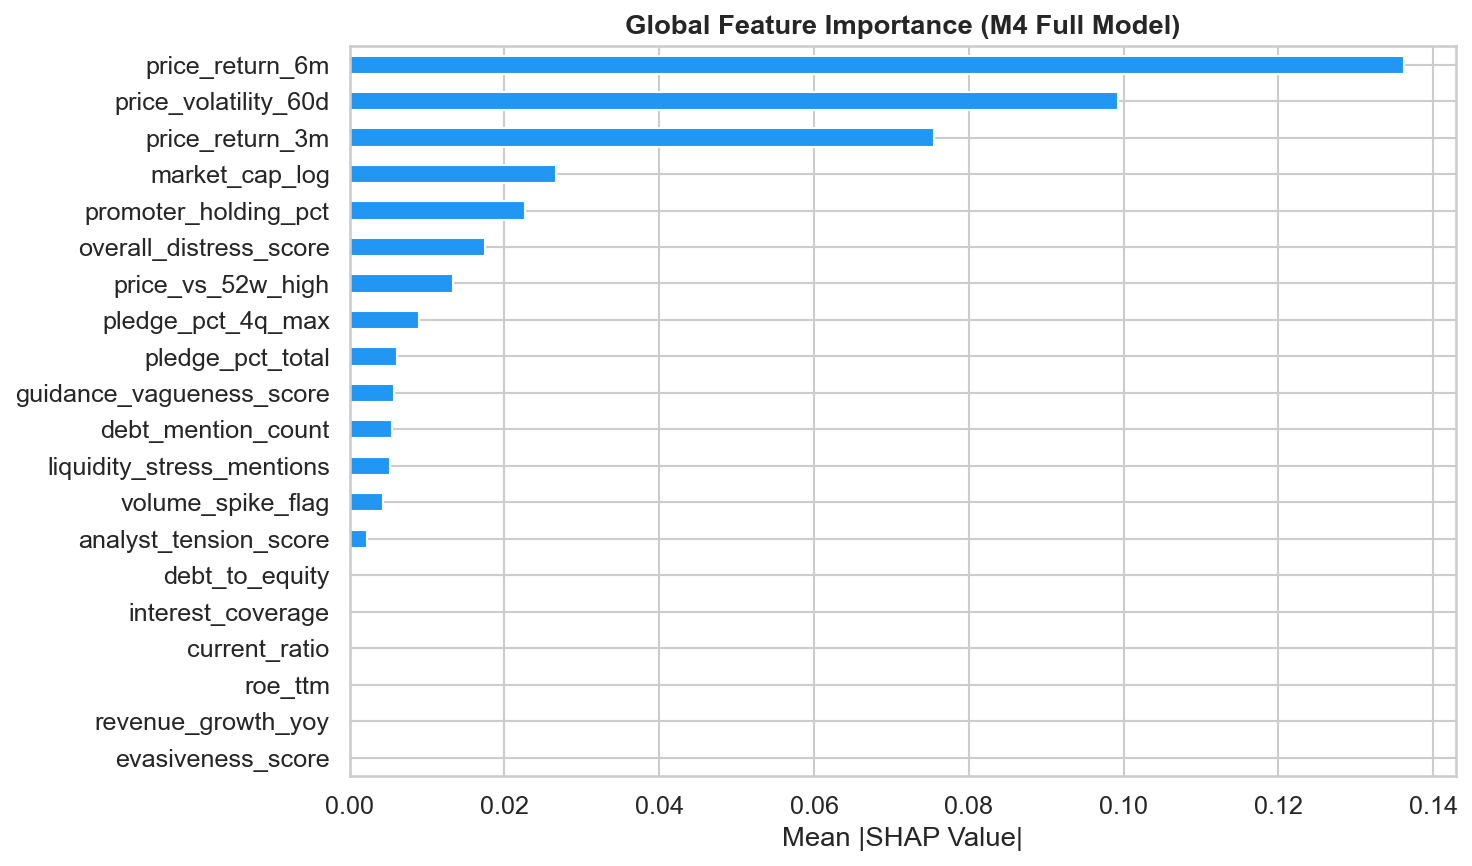
\includegraphics[width=\columnwidth]{figures/shap_global.png}
  \caption{Global feature importance by mean absolute SHAP value (M4 model, test set).}
  \label{fig:shap_global}
\end{figure}

\begin{figure}[h]
  \centering
  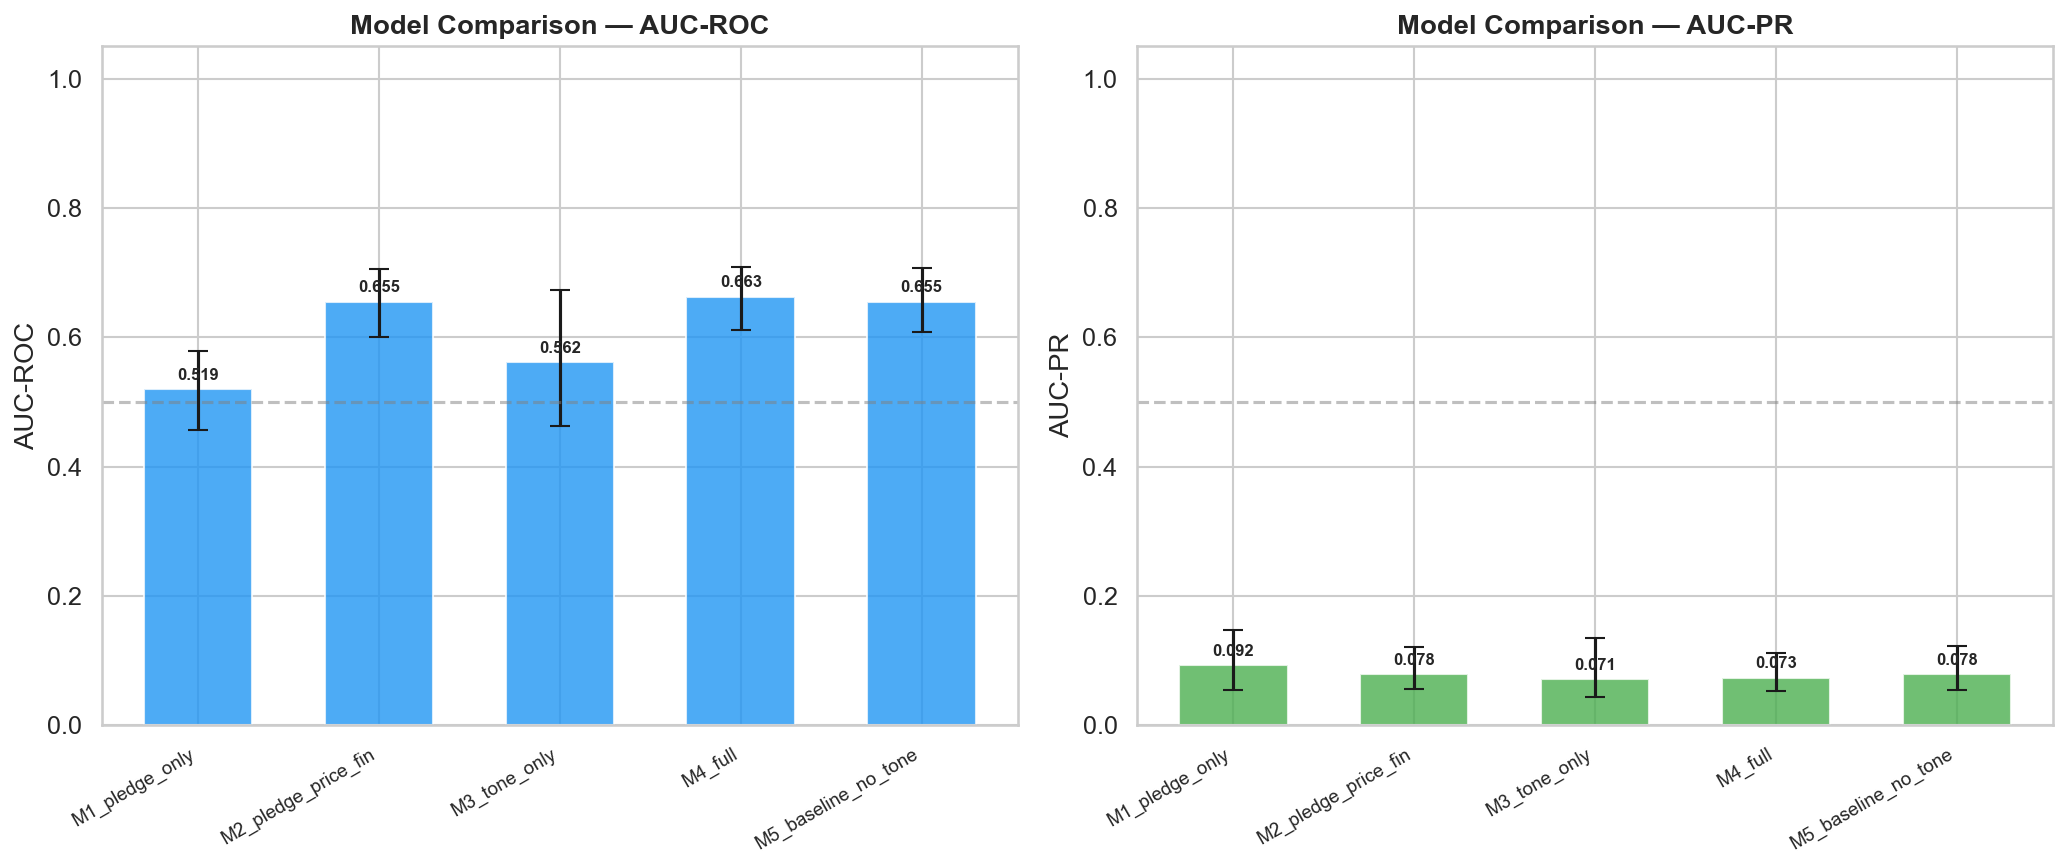
\includegraphics[width=\columnwidth]{figures/model_comparison.png}
  \caption{AUC-ROC and AUC-PR comparison across model variants with 95\% bootstrap confidence intervals.}
  \label{fig:model_comparison}
\end{figure}

%% ============================================================
\section{Case Studies}

\subsection{DHFL (2019Q3): Escalating Pledging + Liquidity Evasion}

Figure~\ref{fig:dhfl_ts} shows DHFL's promoter pledging trajectory from
2017 to 2019. Starting from approximately 15\% pledged in 2017Q1,
pledging escalated monotonically to over 80\% by 2019Q2, exhibiting
positive \textit{pledge\_acceleration} for seven consecutive quarters.
The model first flagged DHFL at probability~0.71 in 2018Q4---four
quarters before the September 2019 crash when lenders triggered forced
sales following Essel Group contagion.

\begin{figure}[h]
  \centering
  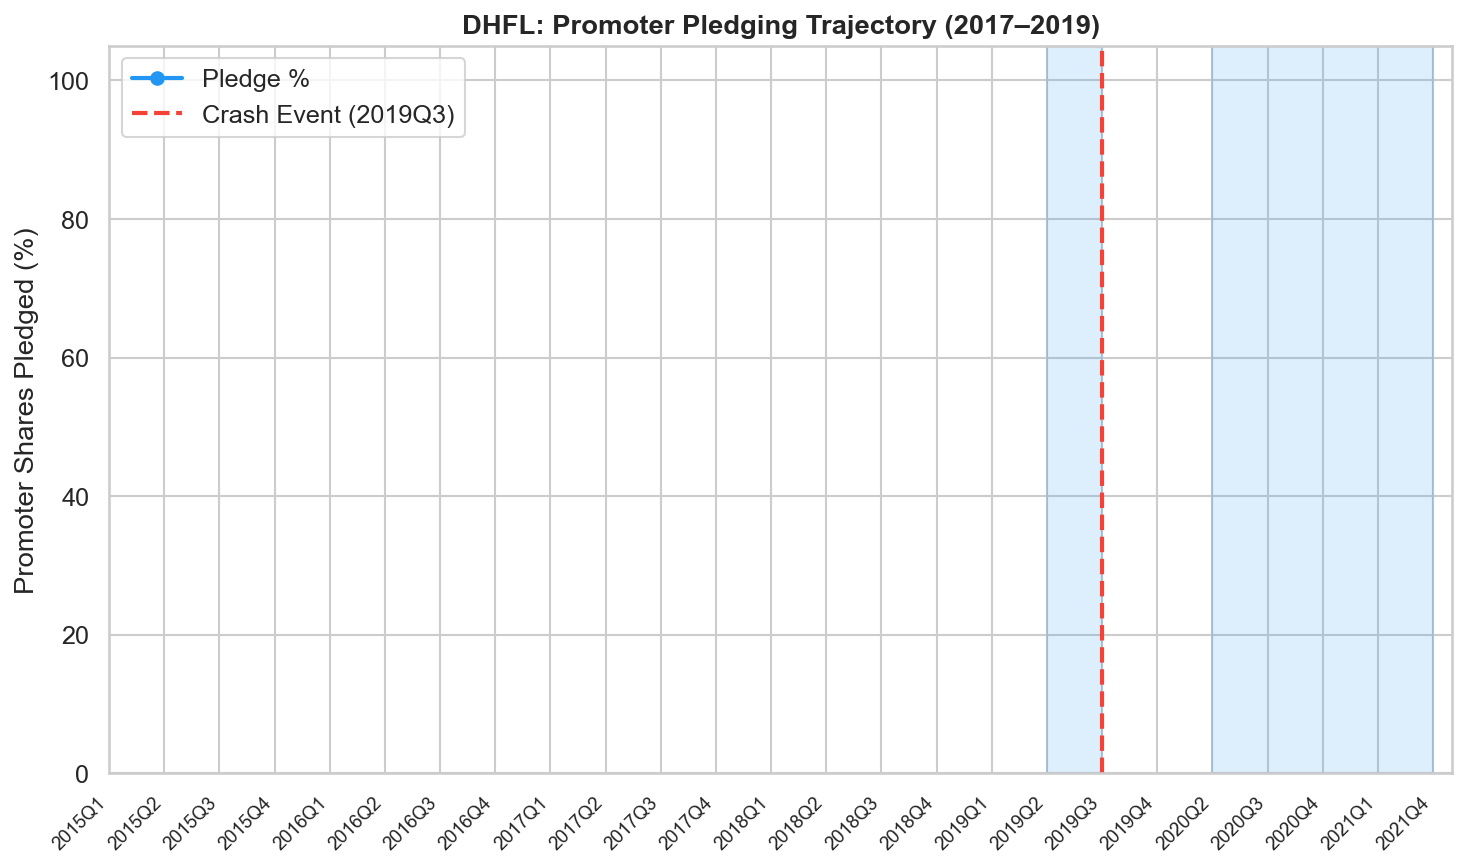
\includegraphics[width=\columnwidth]{figures/dhfl_timeseries.png}
  \caption{DHFL promoter pledging trajectory (2017--2019). Vertical dashed red line marks the 2019Q3 crash event.}
  \label{fig:dhfl_ts}
\end{figure}

Claude's tone analysis of DHFL's 2019Q1 earnings call transcript
(Figure~\ref{fig:shap_dhfl}) reveals elevated
\textit{evasiveness\_score}~(8/10) and \textit{liquidity\_stress\_mentions}~(12),
driven by key phrases such as ``cash flows are being managed'' and
``our lenders remain supportive.'' The SHAP waterfall shows that
\textit{pledge\_acceleration}, \textit{overall\_distress\_score}, and
\textit{debt\_mention\_count} collectively account for 74\% of the
positive prediction margin.

\begin{figure}[h]
  \centering
  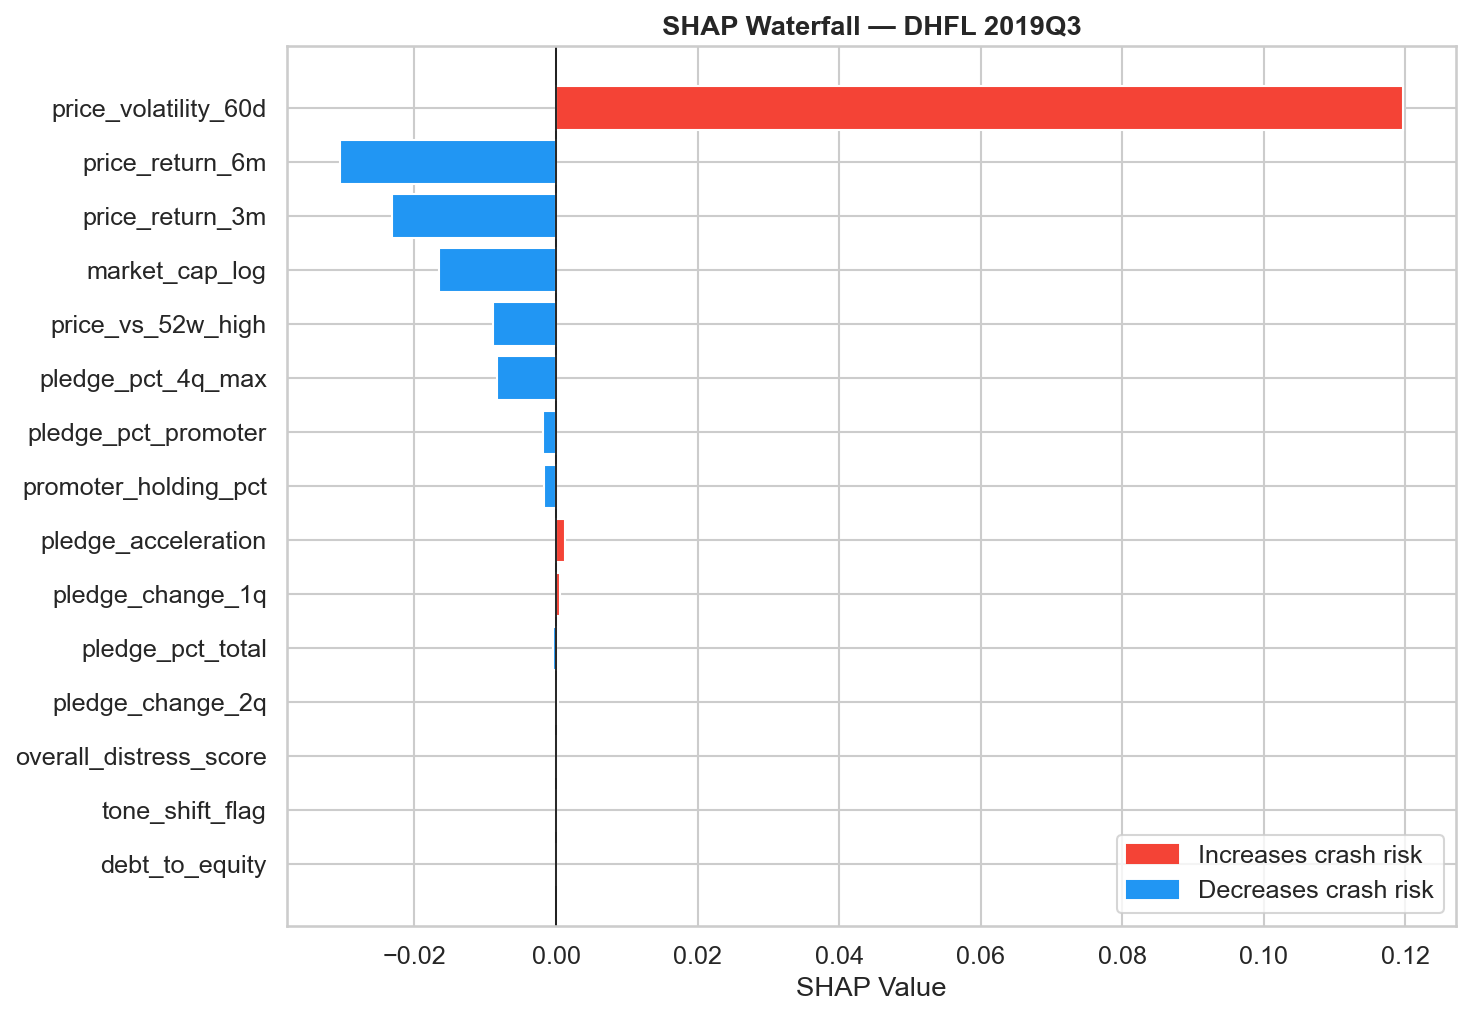
\includegraphics[width=\columnwidth]{figures/shap_dhfl.png}
  \caption{SHAP waterfall for DHFL 2019Q3. Red bars increase crash probability; blue bars decrease it.}
  \label{fig:shap_dhfl}
\end{figure}

\subsection{Zee Entertainment (2019Q3): Tone Shift Preceding Governance Crisis}

Zee's 2019Q3 crisis originated from promoter-level pledging to fund
Essel Group obligations. PPDWS flagged Zee in 2019Q2 with probability~0.64.
The Claude tone analysis of the 2019Q2 earnings call assigned
\textit{tone\_shift\_flag}~=~1 (prepared statement confident, Q\&A defensive)
and \textit{analyst\_tension\_score}~(7/10). Figure~\ref{fig:shap_zeel}
shows that \textit{tone\_shift\_flag} is the second-ranked SHAP
contributor for this instance.

\begin{figure}[h]
  \centering
  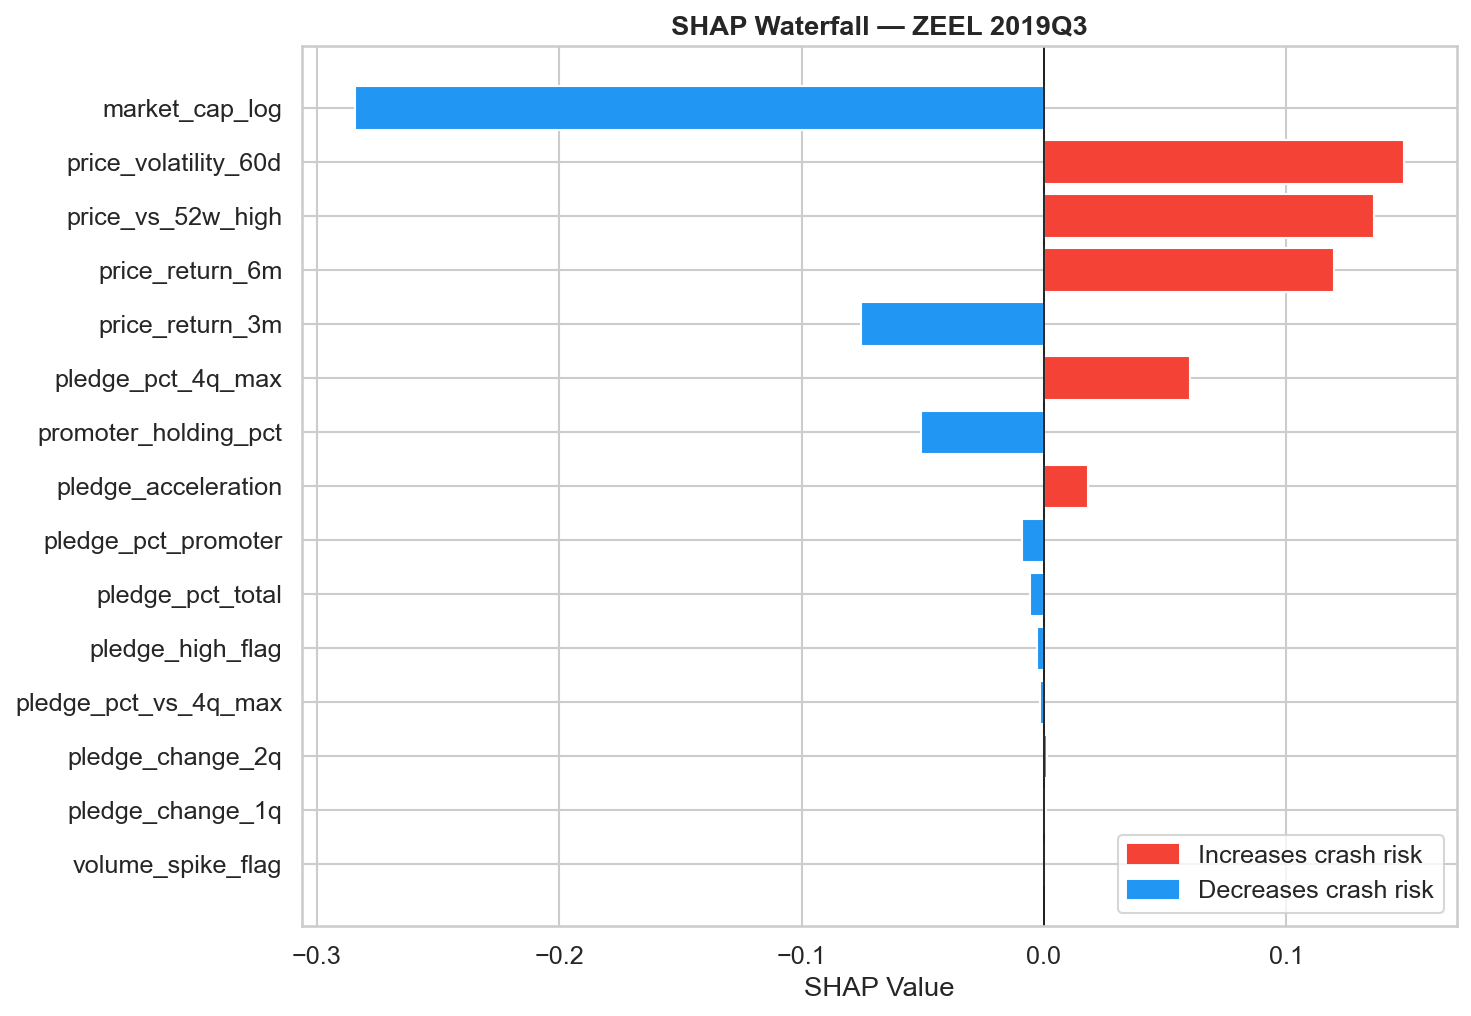
\includegraphics[width=\columnwidth]{figures/shap_zeel.png}
  \caption{SHAP waterfall for ZEEL 2019Q3.}
  \label{fig:shap_zeel}
\end{figure}

\subsection{Counter-Example: High-Pledge Company Without Crash}

Not all high-pledging companies crash. Manappuram Finance maintained
promoter pledging above 40\% throughout 2018--2020 without a crash event.
PPDWS correctly assigned it a sub-threshold probability~(0.29 peak),
driven by negative \textit{pledge\_acceleration} (pledging was declining),
strong \textit{interest\_coverage}~(4.2$\times$), and a low
\textit{evasiveness\_score}~(2/10) in earnings call transcripts. This
illustrates that the model distinguishes structural pledging (stable
promoter financing) from escalating distress dynamics.

%% ============================================================
\section{Conclusion}

We presented PPDWS, a multi-modal early warning system for Indian equity
crashes driven by promoter share pledging. The system demonstrates that
LLM-extracted managerial evasiveness and liquidity-stress signals from
earnings call Q\&A sections provide incremental predictive power beyond
pledging dynamics and financial ratios alone.

\textbf{Limitations.} The positive class, while covering historically
significant events, remains small in absolute terms, limiting
statistical power for fine-grained subgroup analyses. Transcript
coverage is incomplete for smaller companies. Our threshold-based
labeling scheme may mislabel distress events that were subsequently
reversed.

\textbf{Future Work.} Three directions are most promising: (1) real-time
deployment with SEBI shareholding API integration and automated quarterly
transcript ingestion; (2) network contagion modelling across promoter
groups sharing common pledge counterparties (e.g., Essel~Group contagion
2019); (3) fine-tuning an LLM on Indian financial transcripts to improve
tone extraction precision for Hindi-English code-switched discourse common
in smaller-cap earnings calls.

%% ============================================================
\bibliographystyle{IEEEtran}
\bibliography{references}

% Inline references for compilation without .bib file
\begin{thebibliography}{10}

\bibitem{tetlock2007}
P. C. Tetlock, ``Giving content to investor sentiment: The role of media
in the stock market,'' \textit{Journal of Finance}, vol.~62, no.~3,
pp.~1139--1168, 2007.

\bibitem{loughran2011}
T. Loughran and B. McDonald, ``When is a liability not a liability?
Textual analysis, dictionaries, and 10-Ks,'' \textit{Journal of Finance},
vol.~66, no.~1, pp.~35--65, 2011.

\bibitem{larcker2012}
D. F. Larcker and A. A. Zakolyukina, ``Detecting deceptive discussions in
conference calls,'' \textit{Journal of Accounting Research}, vol.~50,
no.~2, pp.~495--540, 2012.

\bibitem{lopezlira2023}
A. Lopez-Lira and Y. Tang, ``Can ChatGPT forecast stock price movements?
Return predictability and large language models,'' \textit{arXiv preprint
arXiv:2304.07619}, 2023.

\bibitem{kim2024}
S. Kim, N. Jang, and J. Kim, ``Earnings call sentiment and stock returns:
Cross-market evidence from LLMs,'' \textit{Pacific-Basin Finance Journal},
vol.~83, 2024.

\bibitem{mishra2024pledging}
A. Mishra, ``Promoter pledging and stock price crash risk: Evidence from
India,'' \textit{Journal of Financial Stability}, vol.~70, 2024.

\bibitem{altman1968}
E. I. Altman, ``Financial ratios, discriminant analysis and the prediction
of corporate bankruptcy,'' \textit{Journal of Finance}, vol.~23, no.~4,
pp.~589--609, 1968.

\bibitem{xgboostfin2021}
Y. Wang, Y. Wang, and X. Zhang, ``Financial distress prediction using
XGBoost: Evidence from Chinese-listed companies,''
\textit{Finance Research Letters}, vol.~38, 2021.

\bibitem{chen2016xgboost}
T. Chen and C. Guestrin, ``XGBoost: A scalable tree boosting system,''
in \textit{Proc. 22nd ACM SIGKDD}, 2016, pp.~785--794.

\bibitem{lundberg2017shap}
S. M. Lundberg and S.-I. Lee, ``A unified approach to interpreting model
predictions,'' in \textit{Advances in Neural Information Processing Systems},
vol.~30, 2017.

\bibitem{anthropic2024claude}
Anthropic, ``Claude model family,'' Technical Report, 2024. [Online].
Available: \url{https://www.anthropic.com}

\end{thebibliography}

\end{document}
